\documentclass{article}
\usepackage[T1]{fontenc}
\usepackage{geometry}
\geometry{a4paper}
\usepackage{setspace}
\usepackage{enumerate}
\usepackage{enumitem}
\usepackage{hyperref}
\usepackage{parskip}
\usepackage[toc]{glossaries}
\hypersetup{colorlinks,allcolors=black,urlcolor=blue}

\setenumerate[1]{itemsep=0pt,partopsep=2pt,parsep=0pt ,topsep=2pt}
\setitemize[1]{itemsep=0pt,partopsep=2pt,parsep=0pt ,topsep=2pt}
\setenumerate[2]{itemsep=0pt,partopsep=2pt,parsep=0pt ,topsep=2pt}
\setitemize[2]{itemsep=0pt,partopsep=2pt,parsep=0pt ,topsep=2pt}
\setdescription{itemsep=0pt,partopsep=2pt,parsep=0pt ,topsep=2pt}

\usepackage{graphicx}
\usepackage{fontspec}

\defaultfontfeatures{%
	RawFeature={%
		% +swsh,
		+calt
	}%
}

\setmainfont{EB Garamond}

\usepackage{multicol}
\usepackage{float}

\usepackage[semibold]{sourcecodepro}

\usepackage{xcolor}
\usepackage{minted}
\usemintedstyle{friendly}

\definecolor{bg}{rgb}{0.95,0.95,0.95}
\newcommand{\codeinline}[1]{
	\mintinline[bgcolor=bg, fontsize=\scriptsize]{text}{#1}
}


\usepackage{relsize}
\newcommand{\bigdataVs}[1]{
	\subsection{#1}
}

\newenvironment{console}{% Caution:
	\VerbatimEnvironment
	\begin{minted}[xleftmargin=2em,bgcolor=bg,fontsize=\small]{console}% Do NOT delete these comments
	}% Otherwise there will be error when compiling
	{%
	\end{minted}%
}
%-----------%

\title{NoSQL Write-up -- Dota2 Game Replay Analysis}
\author{
	Team name: PSG.LGD \\ \\
	Yichun Yan \\
	Ziwei Jiang \\
	Yifan Li \\
	Weiqi Wang
}
\date{\today}


\makeglossaries


\newglossaryentry{Ancient}
{
    name={Ancient},
    description={(also commonly refered to as Thrones, or Tree for Radiant's ancient and Throne for Dire's ancient, as legacy names from DotA) are massive structures found inside each faction's base and are the main objective. In order to win, the enemy team's Ancient must be destroyed, while the own one must be kept alive. Ancients are guarded by their two tier 4 towers. The Ancients are invulnerable until both of their tier 4 towers are destroyed.}
}
\newglossaryentry{MOBA}
{
    name={MOBA},
    description={also known as action real-time strategy (ARTS), is a subgenre of strategy video games that originated as a subgenre of real-time strategy in which each player controls a single character, usually on a map in an isometric perspective, as part of a team competing against another team of players.}
}
\newglossaryentry{professional matches}
{
    name={professional matches},
    description={Matches played two professional teams hosted officially by Valve.}
}
\newglossaryentry{public matches}
{
    name={public matches},
    description={Matches played by ten randomly chosen players, and the results won't influence Matchmaking Rating(MMR) of each player.}
}
\newglossaryentry{ranked matches}
{
    name={ranked matches},
    description={Matches played by ten randomly chosen players according to their Matchmaking Rating(MMR), and the results will influence the Matchmaking Rating of each player.}
}
\newglossaryentry{gold}
{
    name={gold},
    description={Gold is the currency used to buy items or instantly revive your hero. Gold can be earned from killing heroes, creeps, or buildings.}
}
\newglossaryentry{creeps}
{
    name={creeps},
    description={Creeps are basic units in Dota 2. Every unit which is not a hero, building, ward or courier is considered a creep. Creeps can belong to either faction, be neutral, or be player-controlled units. Unlike heroes, creeps do not gain experience and cannot level up. All of their stats are set values (though can still be altered by modifiers). Most creeps grant a set gold and experience bounty to heroes when killed.}
}
\newglossaryentry{XP}
{
    name={XP},
    description={A shorthand for experience. Experience is an element heroes can gather by killing enemy units, or being present as enemy units get killed. On its own, experience does nothing, but when accumulated, it increases the hero's level, so that they grow more powerful. Only heroes can gather experience and therefore reach higher levels. With each level gained, a hero's base attributes increase by static values (unique for each hero), which makes them stronger in several.}
}
\newglossaryentry{match id}
{
    name={match id},
    description={A unique identifier for each match played on Dota2.}
}
\newglossaryentry{sequence number}
{
    name={sequence number},
    description={Similar to match id, which is a unique identifier for each match. But this field will not show up in the Dota2's client.}
}
\newglossaryentry{towers}
{
    name={towers},
    description={Towers are the main line of defense for both teams, attacking any non-neutral enemy that gets within their range. Both factions have all three lanes guarded by three towers each.}
}
\newglossaryentry{barracks}
{
    name={barracks},
    description={Barracks (commonly shortened to Rax) are buildings, defended by their tier 3 towers, that are responsible for keeping lane creeps as powerful as their counterparts.}
}
\newglossaryentry{lane}
{
    name={lane},
    description={A Lane is one of three paths connecting the two Ancients. Lane creeps will push along these lanes after spawning.}
}
\newglossaryentry{AFK}
{
    name={AFK},
    description={A shorthand for away-from-keyboard, AFK means a player leaving a match early before it's end.}
}
\newglossaryentry{buff}
{
    name={buff},
    description={Buffs are positive status effects that enhance your hero.}
}
\newglossaryentry{debuff}
{
    name={debuff},
    description={Debuffs are negative status effects that weaken your hero.}
}
\newglossaryentry{mode}
{
    name={mode},
    description={Game modes are a set of restrictions within which the game of Dota 2 can be played. Most game modes alter how heroes are picked by players. There are also some novelty modes that allow 1v1 play, or give a player a new hero every time they die, for example. }
}
\newglossaryentry{ban}
{
    name={ban},
    description={A ban will disallow the choose for a specific hero within a match.}
}
\newglossaryentry{pick}
{
    name={pick},
    description={A pick is choosing a hero that a player want to play within a match.}
}
\newglossaryentry{first-blood}
{
    name={first-blood},
    description={The first kill within a game. The player who makes the first kill will be rewarded with 150 extra gold}.
}
\newglossaryentry{team battle}
{
    name={team battle},
    description={A battle involves more than half of the players in a match within a short period of time}.
}
\newglossaryentry{buyback}
{
    name={buyback},
    description={While dead, the player has the option to use ``buyback", spending money in order to instantly respawn at the fountain. However, the buyback ability has a long cooldown of 480 seconds and has a scaling gold cost.}.
}
\newglossaryentry{last-hit}
{
    name={last-hit},
    description={You can only get gold from killing creeps or get a kill from killing a hero if you make the last-hit that cause the creeps or hero to death.}.
}
\begin{document}

\maketitle

\tableofcontents
\clearpage

%-------%

\section{Datasets}

\subsection{Background of Datasets}

Our team aims at exploring data about a popular and long-lived computer game, Dota2. Dota2 is a multiplayer online battle arena (\gls{MOBA}) video game developed and published by Valve Corporation. Each game will involve ten players that are divided to two teams play against each other on a same map. Every player chooses one ``hero" that has unique abilities and different styles of playing. The aim for each team is to destroy the building called ``\gls{Ancient}" of the other team. Players collect \gls{gold} to buy powerful items and gain \gls{XP} by killing players on the other team, destroy building of the other team, or kill \gls{creeps}.

\begin{figure}[H]
	\centering
	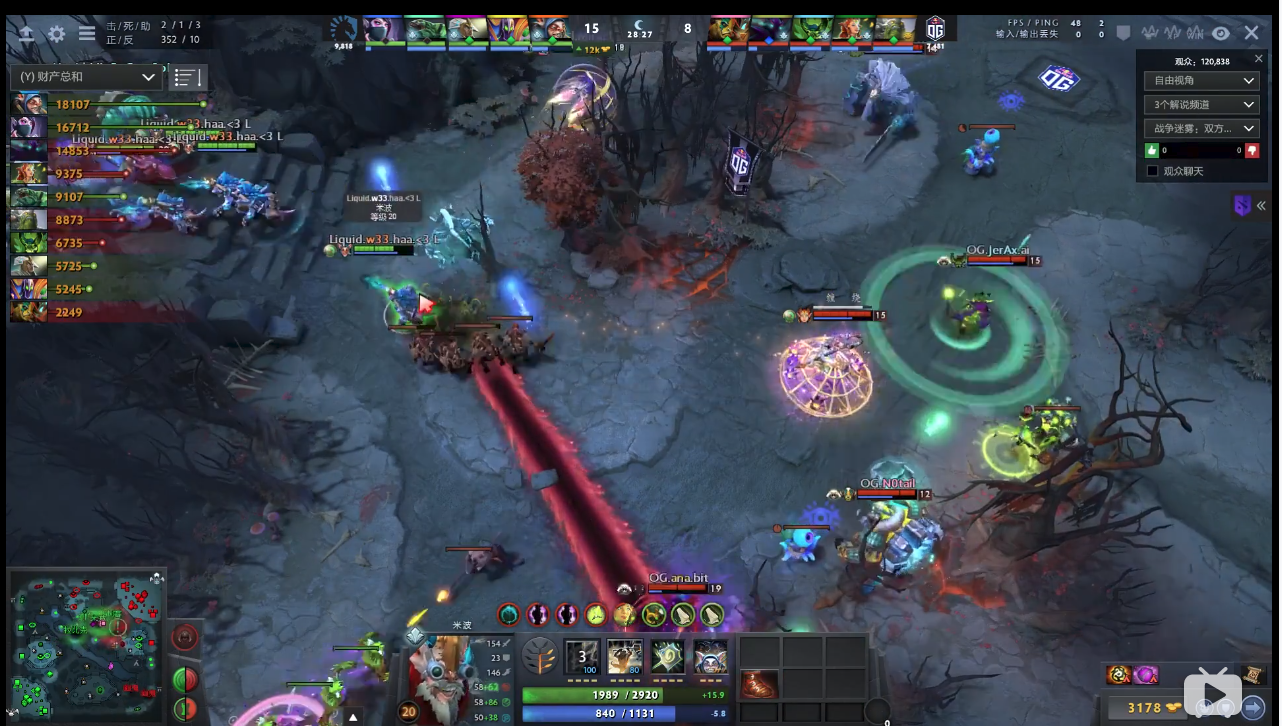
\includegraphics[width=\linewidth]{pic/combat.png}
	\caption{A screenshot of the game}
\end{figure}

It is a real-time game, hundreds of operations and some decisions will be made each second, and all of them will have some influence on the final results of the game. Therefore, there are some professional teams start hiring data engineers to help their players perform better in a game. For example, by using big data pipeline to answer the business question "Does there exist a regular farming path for some professional players?", we can understand both our teammates and the players from other team better, and therefore optimize our strategies.

\subsection{Source of Datasets}

\begin{center}
    \begin{tabular}{|c|c|}
    \hline
    Dataset Name & Dataset Source \\
    \hline\hline
    \href{https://wiki.teamfortress.com/wiki/WebAPI/GetMatchDetails}{Dota2 match result dataset} & \href{https://wiki.teamfortress.com/wiki/WebAPI}{Valve's official API} \\
    \hline
    \href{https://wiki.teamfortress.com/wiki/Replay}{Dota2 replay dataset} & Valve's Dota2 replay servers \\
    \hline
    \end{tabular}
\end{center}

\subsection{Descriptions of Datasets}

\begin{center}
    \begin{tabular}{|p{4.5cm}|p{3.5cm}|p{5cm}|}
    \hline
    Dataset Name & Format & Usage \\
    \hline\hline
    Dota2 match result dataset & JSON & \begin{itemize}
        \item Get match result (containing important information of players and the game such as player name, level, first blood time etc.)
        \item Provide keys for replay dataset
    \end{itemize} \\
    \hline
    Dota2 replay dataset & \codeinline{.dem.bz2} binary file & \begin{itemize}
        \item Get player name, id, team formation and hero choice
        \item Get detail log of the game
        \item Get spawn/death of heros and NPCs
    \end{itemize} \\
    \hline
    \end{tabular}
\end{center}

We will describe how we use Dota2 replay parser to transform different datasets format into usable format in the ETL section.

\subsection{Data Dictionaries}

\section{Data ETL}

\subsection{Extraction}

\subsection{Transformation}

\subsection{Loading}

\subsubsection{Docker}

As mentioned in the proposal, we tried to containerized the project by docker. It is convenient to split up the works for every team mates if we containerized our project. By learning from documents, I tried to configure our project on docker but it ends up with failures. Considering the limited time, we decided to discard using docker for installing our NoSQL technology. However, we learned a lot from this experience.

\begin{enumerate}
    \item Getting Started\\\\
    At this phase, I installed docker, read docker documents, explored docker hub and played around with docker. The objective of this phase is to get familiar with docker and in the end find the way to build the project in Docker way. I learned that we need to build an image, which is an executable package to run the project in the environment of docker. 
    \begin{itemize}
        \item This "package" contains:
        \begin{itemize}
            \item A runtime as a parent image, the overall environment for the container launched by this image;\\(i.e.\codeinline{FROM ubuntu:18.04} from Dockerfile . line2)
            \item Our project code;\\ (i.e.\codeinline{RUN java -jar target/FetchStore.one-jar.jar 4182489531 10 100} from Dockerfile .\ line52)
            \item How we define environment variables;\\ (i.e. \codeinline{ENV JAVA_HOME /usr/lib/jvm/java-8-openjdk-amd64/} from Dockerfile .\ line23)
            \item Installed packages such as java8, maven, mongodb, as the prerequisite of Data ETL;
            \item Working directory set up;\\(i.e.\codeinline{WORKDIR /app} from Dockerfile . line44)
        \end{itemize}
    \end{itemize}
    
    By launching this image, we can get a running container. In other words, a container is an instance of the image. And then we can share our images in a repository on docker hub. When this is done, my teammates can pull and run the image remotely.\\
    
    \item Dockerfile\\\\
    According to the \href{https://docs.docker.com/}{docker documents}, Dockerfile "defines what is going on in the environment inside your container". At the very beginning, I thought dockerize a project just need to pull all the official images in docker, and then we can start manipulate it. But then, after reading documents, I found that we need to construct a Dockerfile to define how a project work, so that it can behaves exactly the same wherever it runs. We can pull an image as a parent image, and then install needed packages in it. \\
    
    For example, in the project, I use ubuntu as a parent image, then docker virtualize an ubuntu operation system environment on your host machine, and then I use Dockerfile as if it is the terminal of ubuntu, writing codes of installing java8, maven, mongodb in the Dockerfile. As mentioned above, then I can use \codeinline{RUN} command to run project code.\\
    
    After I constructed the Dockerfile and try to build the project using \codeinline{$docker build .} in command line, I failed every time when it trying to connect to the database. After reading documents and google for reasons, I realized that it is cramped to put all the service on a Dockerfile. I should construct a docker-compose.yml to define, run and scale service with Docker. \\
    
    \item docker-compose.yml\\
    
    According to our data pipeline, I intended to build 4 services in the docker-compose:\\ 
    \begin{itemize}
        \item Data acquisition and filtering (as "fetchstore" service in the docker-compose, line 17-24)
        \item Data Extraction (as "parsereplay" service in the docker-compose, line 27)
        \item Data Aggregation and Representation (as "mongodb" service in the docker-compose, line 4-16)
        \item Data Analysis (as "analytics" service in the docker-compose, line 29-32)\\
    \end{itemize}
    
    In the docker-compose, we can also use the Dockerfile using the command \codeinline{build} in a service. Therefore, my thought is to construct Dockerfile for "fetchstore", "paresereplay", and "analytics" service using the code and configuration file we have. And use the official image of mongodb, using \codeinline{volume} in the service to reflect the direction of configuration file and mongodb initial javascipt (mogo-init.js, a file to define initial user, database, collections). Also, we used \codeinline{depends_on} to define simple interaction between the services.\\

\end{enumerate}

As the result, we still have a hard time connecting the database. When the problem is fixed, we only finished the configuration of the "fetchstore" service and the "mongodb". Then we realized we got limited time left, therefore, we discard docker for now, and move on to deploy our project on amazon web service (AWS). And we hope to complete this part in the future.

The reason of failure is that I got misunderstanding on Docker's architecture. Also, it is hard for me to consider our system's architecture in Docker's way. And it also need many times of failure to realize the right way to deploy a project on Docker. This experience help us learn how to make the best of documents and google, and also push me to learn a lot about Linux and to read a lot of configuration file.

\section{Data Analysis}

\section{Challenges}



\printglossary

%-------%

\end{document}
